%%%%%%%%%%%%%%%%%%%%%%%%%%%%%%%%%%%%%%%%%%%%%%%%
% E.Pinault-Bigeard - e.pinault-bigeard@upsti.fr
% http://s2i.pinault-bigeard.com
% CC BY-NC-SA 2.0 FR - http://creativecommons.org/licenses/by-nc-sa/2.0/fr/
%%%%%%%%%%%%%%%%%%%%%%%%%%%%%%%%%%%%%%%%%%%%%%%%
\documentclass[11pt]{article}
%%%%%%%%%%%%%%%%%%%%%%%%%%%%%%%%%%%%%%%%%%%%%%%%
% Package UPSTI_Document
%%%%%%%%%%%%%%%%%%%%%%%%%%%%%%%%%%%%%%%%%%%%%%%%
\usepackage{subcaption}
\usepackage[usenames, svgnames, dvipsnames]{xcolor}
\usepackage{UPSTI_Document}
\usepackage{pgfplots}
\definecolor{darkspringgreen}{rgb}{0.09, 0.45, 0.27}

\newcommandx*{\dessinRepereFigGeo}[5][1=\vx{},2=\vy{},3=\vz{},4=,5=0]
	{
		\draw [->,very thick] (0,0) -- (1,0) ;
		\draw [->,very thick] (0,0) -- (0,1) ;
    \fill[white] (0,0) circle (0.13);
    \draw [->,very thick] (0,0) circle (0.13);
    \ifnumequal{#5}{0} {% z vers nous
      \fill[black] (0,0) circle (0.03);
      \draw [->,thick] (0,0) circle (0.04);
    }{% z vers la feuille
  		\begin{scope} [rotate=45]
  			\draw [-,thick] (0,-0.12) -- (0,0.12) ;
  			\draw [-,thick] (-0.12,0) -- (0.12,0) ;
  		\end{scope}
    }
		\draw [anchor=north west] (1.1,0) node {${#1}$};
		\draw [anchor=south west] (0,1.1) node {${#2}$};
		\draw [anchor=north east] (-0.1,0) node {${#3}$};
		\draw [anchor=north west] (-0.1,-0.1) node {${#4}$};
	}

%---------------------------------%
% Paramètres du package
%---------------------------------%

% Version du document (pour la compilation)
% 1: Document prof
% 2: Document élève
% 3: Document à publier
\newcommand{\UPSTIidVersionDocument}{2}

% Variante
%\newcommand{\UPSTIvariante}{2}

% Classe
% 1: PTSI				6: PSI*			11: TSI2		16: Spé
% 2: PT	(par défaut)	7: MPSI			12: ATS
% 3: PT*				8: MP			13: PC
% 4: PCSI				9: MP*			14: PC*
% 5: PSI				10: TSI1		15: Sup
%\newcommand{\UPSTIidClasse}{2}

% Affichage personnalisé de la classe
\newcommand{\UPSTIclasse}{Première STI2D}

% Matière
% 1: S2I (par défaut)    2: IPT     3: TIPE
% 6: Vie au lycée
\newcommand{\UPSTIidMatiere}{4}

% Type de document
% 0: Custom*				7: Fiche Métho de			14: Document Réponses
% 1: Cours (par défaut)		8: Fiche Synthèse    		15: Programme de colle
% 2: TD     				9: Formulaire
% 3: TP						10: Memo
% 4: Colle					11: Dossier Technique
% 5: DS						12: Dossier Ressource
% 6: DM						13: Concours Blanc
% * Si on met la valeur 0, il faut décommenter la ligne suivante:
%\newcommand{\UPSTItypeDocument}{Custom}
\newcommand{\UPSTIidTypeDocument}{3}

% Titre dans l'en-tête
\newcommand{\UPSTItitreEnTete}{Communiquer}
%\newcommand{\UPSTItitreEnTetePages}{UPSTItitreEnTetePages}
%\newcommand{\UPSTIsousTitreEnTete}{UPSTIsousTitreEnTete}

% Titre
%\newcommand{\UPSTItitrePreambule}{Qu'est-ce qu'un réseau ?}
\newcommand{\UPSTItitre}{Nous vivons dans un monde connecté}

% Durée de l'activité (pour DS, DM et TP)
\newcommand{\UPSTIduree}{3h}

% Note de bas de première page
%\newcommand{\UPSTInoteBasDePremierePage}{Note de bas de 1ère page}
% Numéro (ajoute " n°1" après DS ou DM)
%\newcommand{\UPSTInumero}{1}

% Numéro chapitre
\newcommand{\UPSTInumeroChapitre}{5}

% En-tête customisé
%\newcommand{\UPSTIenTetePrincipalCustom}{UPSTIenTetePrincipalCustom}

% Message sous le titre
%\newcommand{\UPSTImessage}{Message sous le titre}

% Référence au programme
%\newcommand{\UPSTIprogramme}{\EPBComp \EPBCompP{B1-02}, \EPBCompP{B2-49}, \EPBCompS{B2-50}, \EPBCompS{B2-51}, \EPBCompP{C1-07}, \EPBCompP{C1-08}}

% Si l'auteur n'est pas l'auteur par défaut
%\renewcommand{\UPSTIauteur}{WWOOOOOOWW}

% Si le document est réalisé au nom de l'équipe
%\newcommand{\UPSTIdocumentCollegial}{1}

% Source
%\newcommand{\UPSTIsource}{UPSTI}

% Version du document
\newcommand{\UPSTInumeroVersion}{1.0}

%-----------------------------------------------
\UPSTIcompileVars		% "Compile" les variables
%%%%%%%%%%%%%%%%%%%%%%%%%%%%%%%%%%%%%%%%%%%%%%%%


%%%%%%%%%%%%%%%%%%%%%%%%%%%%%%%%%%%%%%%%%%%%%%%%
% Début du document
%%%%%%%%%%%%%%%%%%%%%%%%%%%%%%%%%%%%%%%%%%%%%%%%
\begin{document}
\UPSTIbuildPage

\UPSTIobjectif{Ces activités visent à prendre conscience de l'omniprésence des réseaux dans notre entourage.}

\section{Netacad}
Vous avez été inscrits sur un cours de réseau en ligne. Sur la plateforme Netacad, vous aurez accès, pendant 1 an aux ressources de cette séquence, mais aussi des informations plus complètes sur les réseaux.
Tout au long de la séquence, il vous sera demandé de lire des portions du cours en ligne ou de réaliser des TPs. Les synthèses seront faites en classe entière le lundi.

\UPSTIrappel{Le lycée vous fourni une adresse étudiant. Cette adresse est de la forme
\begin{center}
	\UPSTIcadreText{prenom.nom@etudiants.louis-armand.paris}
\end{center}}

\begin{UPSTIactivite}[][Première connexion]
	\begin{itemize}
		\item Connectez-vous sur le site https://www.office.com/
		\item Entrez vos identifiants :
		\begin{description}
			\item [identifiant : ] prenom.nom@etudiants.louis-armand.paris
			\item [Mot de passe : ] Celui donné par le lycée (pour vous connecter à votre session)
		\end{description}
		\item Cliquez sur Outlook : 
\includegraphics[height=.5cm]{Src/Images/outlook}
		\item Ouvrez le mail en provenance de \textbf{Networking Academy} et cliquez sur \textit{Confirmer votre adresse mail}.
		
\includegraphics[height=.7cm]{Src/Images/confirmationmail}
		\item Compléter le formulaire.
		\item Vous devriez maintenant voir apparaitre les cours auxquels vous êtes inscrits. Lancez-le.
	\end{itemize}
\end{UPSTIactivite}

	\begin{figure}[ht]
		\centering
		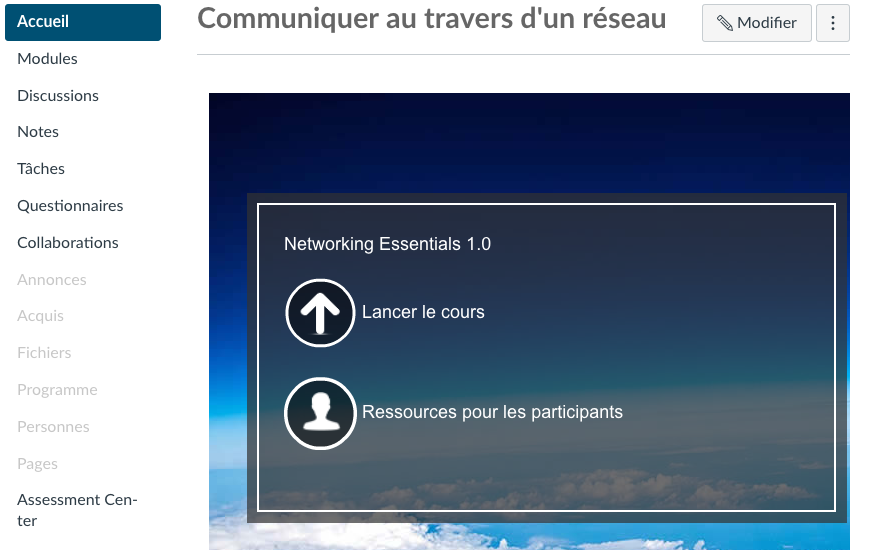
\includegraphics[width=.6\textwidth]{Src/Images/page}
		\caption{Page d'accueil du cours}
		\label{fig:page}
	\end{figure}

	La \UPSTIfig{fig:page} présente la page que vous devriez trouver. Si ce n'est pas le cas, appelez un professeur.

	Sur la gauche, sont accessibles les questionnaires et tâches qui vous seront données. Au centre, c'est le cours à proprement parler. Une fois lancé, le cours se présente sous la forme de figure et de texte associé.

	En ETT et parfois en SIN, vous suivrez les cours de la plateforme CISCO.
	Pour aujourd'hui, nous allons nous concentrer sur certaines activités pratiques autour du réseau.

	Dans la partie latérale, cliquez sur l'onglet 
\includegraphics[height=.5cm]{Src/Images/menuLateral} et cherchez le TP \textbf{TP1 SIN}.

	Une fois les sujets téléchargés, réalisez les deux TPs et répondez aux questions directement sur les documents \textit{.docx} ; ce sont eux que vous rendrez à la fin de la séance. 



\end{document}
